\documentclass[12pt]{article}
\usepackage[utf8x]{inputenc}
\usepackage[serbian]{babel}
\usepackage{geometry}
\usepackage{subcaption}
\usepackage [export]{adjustbox}
\geometry{a4paper} 

\renewcommand{\contentsname}{Sadržaj}
\usepackage{indentfirst}
\usepackage {listings}
\lstset{language=Python}
\usepackage{hyperref}
\begin{document}
\pagenumbering{gobble}
\clearpage

\begin{figure}[h]

\includegraphics[width=0.3\linewidth]{PMF.jpg}

\includegraphics[width=0.3\linewidth,right=10cm]{uns.jpg}
\end{figure}

\begin{center}
{\Large Univerzitet u Novom Sadu\\\Large Prirodno - matematički fakultet,\\ \Large Departman za fiziku}
\end {center}
\begin{center}
\vspace{3.cm}
{\Large  \textbf{INTERPOLACIJA POLJA TEMPERATURE KORISTEĆI PROGRAMSKI JEZIK PYTHON}}
\end {center}
\vspace{1.cm}
\begin{center}
\Large -MASTER RAD-
\end{center}
\vspace{3cm}
\begin{center}Mentor: Prof.dr Ilija Arsenić\hfill Kandidat: Martin Petraš
\end{center}
\vspace{0.5cm}
\begin{center}
Novi Sad, 2018.
\end{center}
\newpage
\pagebreak
\begin{center}
\tableofcontents
\end{center}
\newpage
\pagebreak
\pagenumbering{arabic}
\begin{center}
\section*{Python}
\end{center}
\begin{center}
Programski jezik Python spada u programske jezike visokog nivoa. Njegova sintaksa omogućava pisanje veoma preglednih programa, brzo i lako uči. Programski jezik Python nastao je krajem devedsetih godina prošlog veka. Njegov autor je Gvido van Rosum.Uspeh Python-a se oslanja na nekoliko prednosti koje pruža kako početnicima tako i stručnjacima: Python se lako uči. Broj funkcija u samom jeziku je skroman, pa zahteva relativno malo uloženog vremena ili napora da se naprave prvi programi. Pythonova sintaksa je dizajnirana da bude čitljiva i jednostavna. Ova jednostavnost čini Python idealnim nastavnim jezikom i omogućava početnicima da brzo napreduju. Programeri provode više vremena razmišljajući o problemu koji pokušavaju da reše, a manje vremena razmišljaju o kompleksnosti jezika ili dešifrujući kod koji su pisali drugi. 
Najosnovnije korišćenje Pythona je kao jezik skriptovanja i automatizacije, koristi se za nauku o podacima i mašinsko učenje, za veb usluge, metaprogramiranje. Njegova popularnost se ogleda u velikom broju biblioteka. Što se tiče nedostataka istakli bi njegovu brzinu. Ono za što Pythonu treba šest sekundi u drugom programskom jeziku se može uraditi za delić sekunde. Međutim, brzina kojom se može napisati funkcionalan program je daleko brži nego u nekom drugom jeziku.  
\end{center}
\newpage
\begin{center}
\section*{Uvod}
U ovom radu biće predstavljeno kako uz pomoć Pythona i njegove biblioteke Metpy možemo nacrtati polje temperature. Konkretno će obrađenja oblast u području planina Karpati. Biće pokazano kako instalirati odgovarajuće biblioteke potrebene za rad. Osvrnućemo se i na postupak interpolacije koji je korišćen kod metpy biblioteke. Prvi deo rada obuhvatiće postupke za konfigurisanje a u drugom delu će biti predstavljeni rezultati. 
\end{center}
\newpage
\section{Postupak za instaliranje}
Python kao programski jezik postoji za sve tri popularne sistemske platforme Windows,Linux i OSX. Ovde će biti prikazan postupak instaliranja potrebnih paketa za rad pod Linux operativnim sistemom. Konkretno ćemo raditi na distribuciji baziranoj na Debian(stable) paketima, međutim za ostale distribucije poput Suse, Fedora, Arch postupak je sličan.
Prvo što treba da uradimo jeste da odemo na \url{https://www.anaconda.com/download/#linux} i preuzmemo $Anaconda3-5.2.0-Linux-x86{\_64}.sh$\footnote{U pitanju je trenutna verzija}. U pitanju je \textsl{shell} skripta koja se pokreće u terminalu na sledeći način: 
\begin{lstlisting}
 bash Anaconda3-5.2.0-Linux-x86_64.sh
\end{lstlisting}
Nakon što se prihvati licenca određujemo gde da instaliramo Anacondu, najbolje je da se ostavi podrazumevana putanja $/home/USER/anaconda$. Nakon završene instalacije najbolje je uraditi modifikaciju \textsl{.bashrc} dodavanjem sledeće putanje:
\begin{lstlisting}
 export PATH=/home/$USER/anaconda/bin:$PATH
\end{lstlisting}
Nakon ovoga uspešno smo instalirali anacondu koju ćemo koristi za instaliranje odnosno ažuriranje Python paketa. Paketi se uz pomoć Anaconde instaliraju upisivanjem sledeće komande u terminal:
\begin{lstlisting}
 conda install ime_paketa 
\end{lstlisting}
Za ažuriranje paketa koristi se sledeća komanda:
\begin{lstlisting}
 conda update ime_paketa 
\end{lstlisting}
Postoji još jedan metod kojim se mogu instalirati paketi, a to je uz pomoć komande \textsl{pip}:
\begin{lstlisting}
 pip install ime_paketa 
\end{lstlisting}
Međutim, jako bitno je istaći da ne treba mešati ova dva metoda za instaliranje paketa. Najbolje je da se izabere jedan od njih i uvek koristi, jer mogu nastati problemi ako se koriste oba metoda. 
 \subsection{Provera verzije pythona}
Prvo proveravamo da li imamo instaliran python kucanjem sledeće komande:
\begin{lstlisting}
 python 
\end{lstlisting}
Ukoliko je python instaliran pojavi se sledeće
\begin{figure}[h!]
\centering
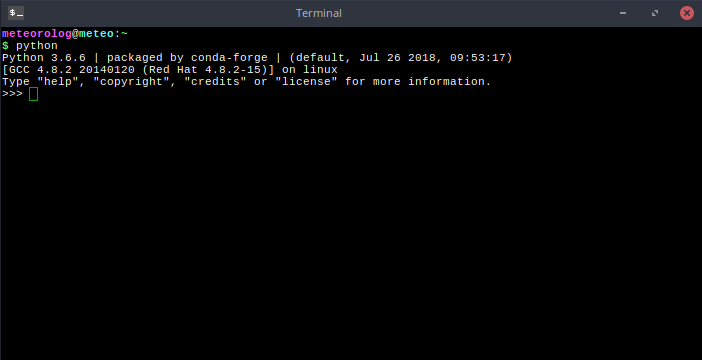
\includegraphics[width=1.\linewidth]{python.png}
\caption*{\textsl{Slika 1. Pokretanje pythona}}
\end{figure}
Uglavnom sve distribucije linuxa dolaze sa instaliranim pythonom, razlika može biti u verziji. Postoje dve verzije pythona, 2.7 čija podrška polako prestaje i novija 3.x (trenutna je 3.6.6). Razlike između ove dve verzije postoje, ali metpy biblioteka koja nama je potrebna podržava obe verzije. Više o razlikama između ove dve verzije pogledajte na \url{https://wiki.python.org/moin/Python2orPython3}. Koja verzija pythona je instalirana možemo proveriti i kucanjem sledećeg koda u terminal:
\begin{lstlisting}
 python --version
 Python 3.6.6
\end{lstlisting}  
U buduće svaki kod će biti vezan za ovu verziju.
\subsection{Izbegavanje problema sa dve verzije}
Kao što sam već spomenuo sve linux distribucija dolaze sa instaliranim pythonom, razlike mogu biti u verziji. Ukoliko vaša linux distribucija ima instaliranu samo verziju 2.7 a vi bi hteli i verziju 3.x, onda treba obratiti pažnju na sledeće. Kod mene, ja koristim MX linux distribuciju baziranu na Debian(stable) verziji, kucanjem u terminalu:
\begin{lstlisting}
 python --version
 Python 3.6.6
\end{lstlisting}  
\begin{figure}[h!]
\centering
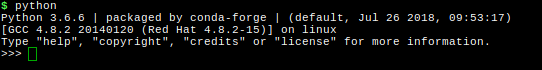
\includegraphics[width=1.\linewidth]{python3.png}
\caption*{\textsl{Slika 2. Pokretanje pythona verzije 3.6.6}}
\end{figure}
prikazuje da je podrazumevana verzija 3.6. Međutim, ukoliko je kod vas instalirana samo verzija 2.7 a vi dodatno instalirante verziju 3.x, može se desiti da će verzija 2.7 i dalje ostati podrazumevana, pa se prilikom kompajliranja može javiti problem. Pošto su kod mene obe vezije, kao podrazumevana verzija je 3.6.6 dok je za pozivanje verzije 2.7 potrebno kucati sledeće:
\begin{lstlisting}
 python2 --version
 Python 2.7.13
\end{lstlisting}
\begin{figure}[h!]
\centering
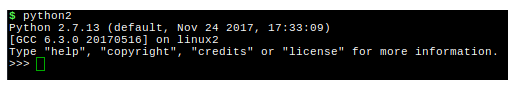
\includegraphics[width=1.\linewidth]{python2.png}
\caption*{\textsl{Slika 3. Pokretanje pythona verzije 2.7}}
\end{figure}
  Kako bi otklonili ovaj problem, u direktorijumu \textsl{/home/user/.bashrc}, koristeći jedna od tekst editora, upišemo sledeću komandu:
\begin{lstlisting}
 alias python=python3
\end{lstlisting}  
Ovom komandom prilikom svakog pozivanja pythona iz terminala kao podrazumevana verzija će biti 3.6.6, što će biti jako bitno u daljem radu.
 \section{Korišćenje biblioteka}
Mnoge python funkcije su sadržane u specijalizovanim bibliotekama, tzv. modulima. Kako bi se ove funkcije mogle koristiti, one se moraju učitati. Učitavanje modula se postiže naredbom \textsl{import}. Ova mogućnost je pythonu donela popularnost jer postoje monogo modula koji jako pomažu prilikom rada. Python je provo svoju popularnost stekao pri izradi veb programa međutim usavršavanjem podrške za dodtane module otvorilo je vrata pythonu i u drugim oblastima. Moduli poput \textsl{numpy} i \textsl{pandas}, koji se koriste za analizu i vizuelno prikazivanje podataka, su python svrstali uz rame sa ostalim kako komercijalnim programima tako i sa programima otvorenog koda kao što su R, MATLAB, SAS, Stata i ostali. Kada pogledamo da python spada u besplatni programski jezik, njegova popularnost nije slučajnost. Jedan deo ove popularnosti u obradi podataka pripada i laka integracija sa C, C++ i FORTRAN kodom.  
Pošto su moduli jako značajni za python istaći ćemo neke od naznačajnijih. Samo da napomene, sve nabrojane mogućnosti koje pružaju biblioteke je moguće izvesti koristeći isključivo samo Pythonov kod. Prednost biblioteka je u efikasnosti i lakoći kojim se postižu isti rezultati, uz manje utrošenog vremena.  
\subsection{NumPy}
NumPy (Numerical Python) je jedan od glvanih modula koji se koristi za numeričke proračune u pythonu. Sadrži sledeće stvari:
\begin{itemize}
\item objekt \textsl{ndarray}, brz i efikasan višedimenzioni niz
\item sadrži funkcije za brzi rad sa redovima
\item alate za čitanje i pisanje nizova iz dadoteka
\item operacije sa linearnom algebrom, Furijeve transformacije, nasumično kreiranje brojeva
\item omogućava interakciju sa C i C++ kodom 
\end{itemize}
Za numeričke proračune, nizovi kod NumPy su dosta efikasniji prilikom njihove manipulacije nego bilo koja druga izgrađena struktura unutar Pythona. Instaliranjem Anaconde ova biblioteka bi trebalo da bude instalirana, ukoliko to nekim slučajem nije, to se radi na sledeći način:
\begin{lstlisting}
 conda install numpy
\end{lstlisting}
Ukoliko želimo ažurirati novu verziju:
\begin{lstlisting}
 conda update numpy
\end{lstlisting}
\subsection{Pandas}
Pandas je dizajniran kako bi se ubrzao rad sa strukturiranim ili tabelarnim podacima i kao takav, postao jako moćna i produktivna alatka za analizu podataka. Sadrži sve osobine NumPy s mogućnošćom brže i efikasnije manupulacije bazom podataka. Brzo i lako indeksiranje, preoblikovanje, sečenje, spajanje, brisanje su samo od nekih mogućnosti koje pruža ova biblioteka u radu sa podacima. Instaliranje pandas biblioteke:
\begin{lstlisting}
 conda install pandas
\end{lstlisting}
\subsection{MetPy}
Metpy predstavlja kolekciju alata u Pythonu za pregled, vizuilizaciju i proračuna meteoroloških podataka. Paket je nastao od strane \textsl{Unidata} udruženja, koja se bavi izradom alata za naučne svrhe. MetPy paket sadrži dosta opcija, koristi se za vizelizaciju radarskih slika, rad sa netCDF podacima,vizuelizaciju radio-sondažnih merenja, vizuelizaciju meteoroloških podataka i ostalo. Mi ćemo koristi ovu biblioteku u svrhu interpolacije polja temperature. Za instaliranje MetPy u terminal kucamo:
\begin{lstlisting}
 conda install -c -conda-forge metpy
\end{lstlisting}
Instaliranjem ovog paketa dobijamo razne alate, nama će najviše značiti mogućnost interpolacije za polje temperature kao i negove vizuelizacije. Za vizuilizaciju se koristi \textsl{Cartopy}, Pythonov paket za crtanje mapa.


\end{document}
